\section{Declarative Programmable Storage}
\label{sec:prog-model}

\begin{figure*}[t]
\begin{subfigure}{.8\columnwidth}
    \centering
    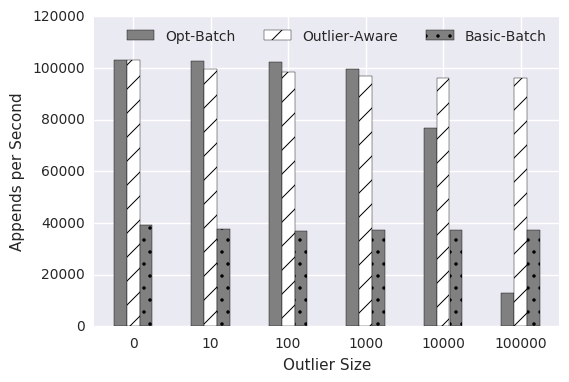
\includegraphics[width=0.95\columnwidth]{batching-outlier-detect.png}
    \caption{}
    %\caption{Identifying and handling an outlier independently maintains the
    %beneifts of batching without the performance degredation of unecessarily
    %large I/O requests.}
    \label{fig:batching-outlier}
\end{subfigure}\hfill
\begin{subfigure}{.3\columnwidth}
\centering
\scalebox{.6}{
\begin{tikzpicture}[->,>=stealth',shorten >=1pt,auto,node distance=2.2cm,semithick]
%\tikzstyle{every state}=[fill=red,draw=none,text=white]

  \node[initial left,state] (A)              {$EG$};
  \node[state]         (B) [below left of=A] {$CP$};
  \node[state]         (D) [below of=B]       {$IO$};
  \node[state]         (C) [below right of=A] {$GC$};
  \node[state]         (E) [below of=C]       {$US$};
  \node[state]         (F) [below left of=E] {$Out$};

  \path (A) edge        node [left] {R,W,F} (B)
            edge        node {T}     (C)
        (B) edge        node {F}     (C)
            edge        node {R,W}   (D)
        (C) edge        node {F,T}   (E)
        (D) edge        node {W}     (E)
            edge        node {R}     (F)
        (E) edge        node {F,T,W} (F);
\end{tikzpicture}
}
\caption{}
\label{fig:corfu-sm}
\end{subfigure}\hfill
\begin{subfigure}{.65\columnwidth}
\centering
\includegraphics[width=0.95\columnwidth]{Corfu_viz_expanded3.pdf}
\caption{}
\label{fig:dataflow}
\end{subfigure}
\caption{(a) batching performance with and without outlier detection (b) state
machine for the CORFU storage device. (c) logical dataflow of the
CORFU storage protocol which could not be more concise and still capture the
state machine.}
\label{fig:pm}
\end{figure*}

Current ad-hoc approaches to programmable storage restrict
use to developers with distributed programming expertise, knowledge of the
intricacies of the underlying storage system and its performance model, and
use hard-coded imperative methods. This limits the use of optimizations that
can be performed automatically or derived from static analysis.  Based on the
challenges we have demonstrated stemming from the dynamic nature and large
design space of programmable storage, we propose an alternative, declarative
programming model which reduces the learning curve for new users, and allows
existing developers to increase productivity by writing fewer, more portable lines of code.

The model we propose corresponds to a subset of Bloom, a
declarative language for expressing distributed programs as an unordered set
of rules~\cite{alvaro:cidr11}. Bloom rules fully specify program semantics and
allow developers to ignore the details associated with program
evaluation. This level of abstraction is attractive for building storage
interfaces whose portability and correctness is critical. We use Bloom to model the
storage system state uniformly as a collection of relations, with interfaces
expressed as a collection of \emph{queries} over a request stream that
are filtered, transformed, and combined with other system state. We present a
brief example of the CORFU shared-log interface expressed using this model.

\subsection{Example: CORFU as a Query}

We model the storage interface of the CORFU protocol as a query in our
declarative language in which shared-log and other metadata are represented by
two persistent abstract collections mapped onto physical storage. This
transformation permits optimizations and implementation details (e.g. log
striping and partitioning) to be discovered and applied transparently by an
optimizer.  Since the specification of the interface is invariant across
system changes and low-level interfaces, the optimizer can automatically
render execution decisions and build indexes using the performance
characteristics of specific access methods.  For example a low-level indexing
engine for text will likely be out-performed by other engines for the CORFU
64-bit write-once address space interface.  Likewise, an instance of the
interface that uses fixed log entries can directly map log entries onto a
low-level byte stream, avoiding an explicit index in some situations.

Amazingly, the semantics of the entire storage interface requirements in
CORFU\footnote{Due to space limitations refer to \cite{watkins:ucsc-soe-16-12}
for a full program listing.} are expressible using only a few Bloom code
snippets amenable as input to an optimizer.  Figure~\ref{fig:corfu-sm}
shows the state transition diagram for the CORFU storage interface and
Figure~\ref{fig:dataflow} shows the corresponding dataflow diagram for the
Bloom CORFU protocol. Beyond the convenience of writing less code, the
entire experience of designing and writing an interface such as CORFU in a
declarative language such as Bloom eases the process of constructing
convincingly correct implementations. Specifically, the high-level details
of the implementation mask distracting issues related to the physical
design and the many other ``gotchas'' associated with writing low-level
systems software.

Our current Bloom specification of the CORFU protocol assumes the existence of
an external sequencer service to assign log positions. However, we are working
towards a specification that defines the sequencer service as a view over the
log, whose state is managed in volatile storage. A declarative specification
will be critical to providing portability of the service, since storage
systems internally utilize volatile storage in many forms (e.g. memory caches
and non-replicated data). For example, our work in Malacology showed how inode state in a
distributed file system could be used to build a sequencer,
but an object-based storage system could place sequencer
state in an object cache while providing fast-path access that is difficult to
achieve with the consistency and durability requirements of non-volatile
object state.

%In addition, the CORFU interface depends on a trim
%interface to mark unused poritions of the log (shown on lines 10-15) Trimmed
%entries are tracked as unused for reclamation, and implementations may take
%advantage of specific optimizations provided by an index implementation or
%hardware support found in modern non-volatile memories.

%\begin{lstlisting}[caption={Sample \emph{corfu.bloom} program listing}, label=lst:corfublm]
%bloom :corfu do
%  table :epoch, [:epoch]
%  table :log, [:pos] => [:state, :data]
%  scratch :write_op, op.schema
%end
%bloom :write do
%  temp :valid_write <= write_op.notin(found_op)
%  log <+ valid_write{|o| [o.pos, 'ok', o.data]}
%  ret <= valid_write{|o| [o.type, o.pos, o.epoch, 'ok'] }
%  ret <= write_op.notin(valid_write) {|o| ['read-only'] }
%end
%bloom :trim do
%  log <+- trim_op{|o| [o.pos, 'trimmed']}
%  ret <=  trim_op{|o|
%    [o.type, o.pos, o.epoch, 'ok']}
%end
%\end{lstlisting}


%\begin{figure}
%\centering
%\includegraphics[width=0.7\columnwidth]{Corfu_viz_expanded2.png}
%\caption{Dataflow graph for the CORFU interface written in Bloom}
%\label{fig:flow}
%\end{figure}


%For reference our prototype implementation of CORFU in Ceph (called
%ZLog\footnote{https://github.com/noahdesu/zlog}) is written in C++ and the
%storage interface component comprises nearly 700 lines of code, and uses a
%hard-coded indexing strategy that has been rewritten multiple times to explore
%alternative optimization techniques.

%\begin{figure}[t]
%\begin{subfigure}{.2\columnwidth}
%\centering
%\scalebox{0.4}{
%\begin{tikzpicture}[->,>=stealth',shorten >=1pt,auto,node distance=2.2cm,semithick]
%%\tikzstyle{every state}=[fill=red,draw=none,text=white]
%
%  \node[initial left,state] (A)              {$EG$};
%  \node[state]         (B) [below right of=A] {$CP$};
%  \node[state]         (D) [right of=B]       {$IO$};
%  \node[state]         (C) [above right of=A] {$GC$};
%  \node[state]         (E) [right of=C]       {$US$};
%  \node[state]         (F) [below right of=E] {$Out$};
%
%  \path (A) edge        node [left] {R,W,F} (B)
%            edge        node {T}     (C)
%        (B) edge        node {F}     (C)
%            edge        node {R,W}   (D)
%        (C) edge        node {F,T}   (E)
%        (D) edge        node {W}     (E)
%            edge        node {R}     (F)
%        (E) edge        node {F,T,W} (F);
%\end{tikzpicture}
%}
%\caption{}
%\label{fig:corfu-sm}
%\end{subfigure}\hfill
%\begin{subfigure}{.6\columnwidth}
%\centering
%\includegraphics[width=1.0\columnwidth]{Corfu_viz_expanded.png}
%\caption{}
%\label{fig:malacologyx}
%\end{subfigure}
%\end{figure}

%\begin{figure*}[t]
%\begin{subfigure}{.3\columnwidth}
%\centering
%\scalebox{0.45}{
%\begin{tikzpicture}[->,>=stealth',shorten >=1pt,auto,node distance=2.2cm,semithick]
%%\tikzstyle{every state}=[fill=red,draw=none,text=white]
%
%  \node[initial left,state] (A)              {$EG$};
%  \node[state]         (B) [below right of=A] {$CP$};
%  \node[state]         (D) [right of=B]       {$IO$};
%  \node[state]         (C) [above right of=A] {$GC$};
%  \node[state]         (E) [right of=C]       {$US$};
%  \node[state]         (F) [below right of=E] {$Out$};
%
%  \path (A) edge        node [left] {R,W,F} (B)
%            edge        node {T}     (C)
%        (B) edge        node {F}     (C)
%            edge        node {R,W}   (D)
%        (C) edge        node {F,T}   (E)
%        (D) edge        node {W}     (E)
%            edge        node {R}     (F)
%        (E) edge        node {F,T,W} (F);
%\end{tikzpicture}
%}
%\caption{}
%\label{fig:corfu-sm}
%\end{subfigure}\hfill
%\begin{subfigure}{.5\columnwidth}
%\centering
%\includegraphics[width=0.95\columnwidth]{Corfu_viz_expanded.png}
%\caption{}
%\label{fig:malacologyx}
%\end{subfigure}\hfill
%\begin{subfigure}{0.9\columnwidth}
%
%\begin{lstlisting}[title={{\bf (c)}}, label=lst:write]
%bloom :write do
%  temp :valid_write <= write_op.notin(found_op)
%  log <+ valid_write{ |o| [o.pos, 'valid', o.data]}
%  ret <= valid_write{ |o|
%    [o.type, o.pos, o.epoch, 'ok'] }
%  ret <= write_op.notin(valid_write) {|o|
%    [o.type, o.pos, o.epoch, 'read-only'] }
%end
%\end{lstlisting}
%\end{subfigure}
%\caption{foo}
%\end{figure*}

